\hsection{Example: Layout of Factories}%
%
There are both dynamic and static aspects of intelligent production, as well as all sorts of nuances in between.
The question of where to put which facility in a factory is a rather static, but quite important aspect.
Let us assume we own a company and bought a plot of land to construct a new factory.
Of course we know which products we will produce in this factory.
We also know which facilities we need to construct, i.e., the workshops, storage depots, and maybe an administrative building.
What we need to decide is where to place them on our land, as illustrated in \autoref{fig:qap_example}.%
%
\begin{figure}%
\centering%
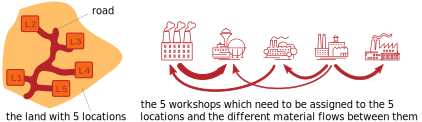
\includegraphics[width=0.99\linewidth]{\currentDir/qap_example}%
\caption{Illustrative sketch of a quadratic assignment scenario, where different buildings of a factory need to be laid out on a plot of land.}%
\label{fig:qap_example}%
\end{figure}%

Let us assume we have $n$~locations on our plot of land that we can use for our $n$~facilities.
In some locations, there might be already buildings, in others, we may need to construct them anew.
For each facility and location pair, a different construction cost may arise.
A location with an existing shed might be a good solution to put a warehouse.
However, if we want to put the administration building there, we would first need to demolish the shed.
These are the static costs.

But placing the facilities also has a very big impact on the running costs.

For every possible plan, costs also arise from the relative distances between the facilities that we wish to place.
Maybe there is a lot of material flow between two of the workshops.
Finished products and raw material may need to be transported between a workshop and the storage depot.
Between the administration building and the workshops, on the other hand, there will usually be no material flow.
Of course, the distance between two facilities will depend on the locations we pick for them.
For each pair of facilities that we place on the map, flow costs will arise as a function of the amount of material to be transported between them and the distance of their locations.

The total cost of an assignment of facilities to locations is therefore the sum of the resulting base costs and flow costs.
Our goal would be to find the assignment (i.e., the plan) with the smallest possible total cost.

This scenario is called \emph{quadratic assignment problem}~(QAP)~\cite{BCPP1998TQAP}.
It has been subject to research since the 1950s~\cite{BK1957APATLOEA}.
QAPs appear in wide variety of scenarios such as the location of facilities on a plot of land or the placement of work stations on the factory floor.
Even if we need to place components on a circuit board in a way that minimizes the total wire length, we basically have a QAP, too~\cite{S1961TBWPAPA}!
Despite being relatively simple to understand, the QAP is hard to solve~\cite{SGA1976PCAP}.
%
\endhsection%
%
